\section{Storage Element: Flip-Flops}
\label{sec:stor-ele-flip-flop}

Flip-flop circuits are constructed in such a way as to make them operate properly when they are part of a sequential circuit that employs a common clock. The problem with the latch is that it responds to a change in the \textit{level} of a clock pulse. The key to the proper operation of a flip-flop is to trigger it only during a signal \textit{transition}.

\begin{figure}[H]
  \centering
  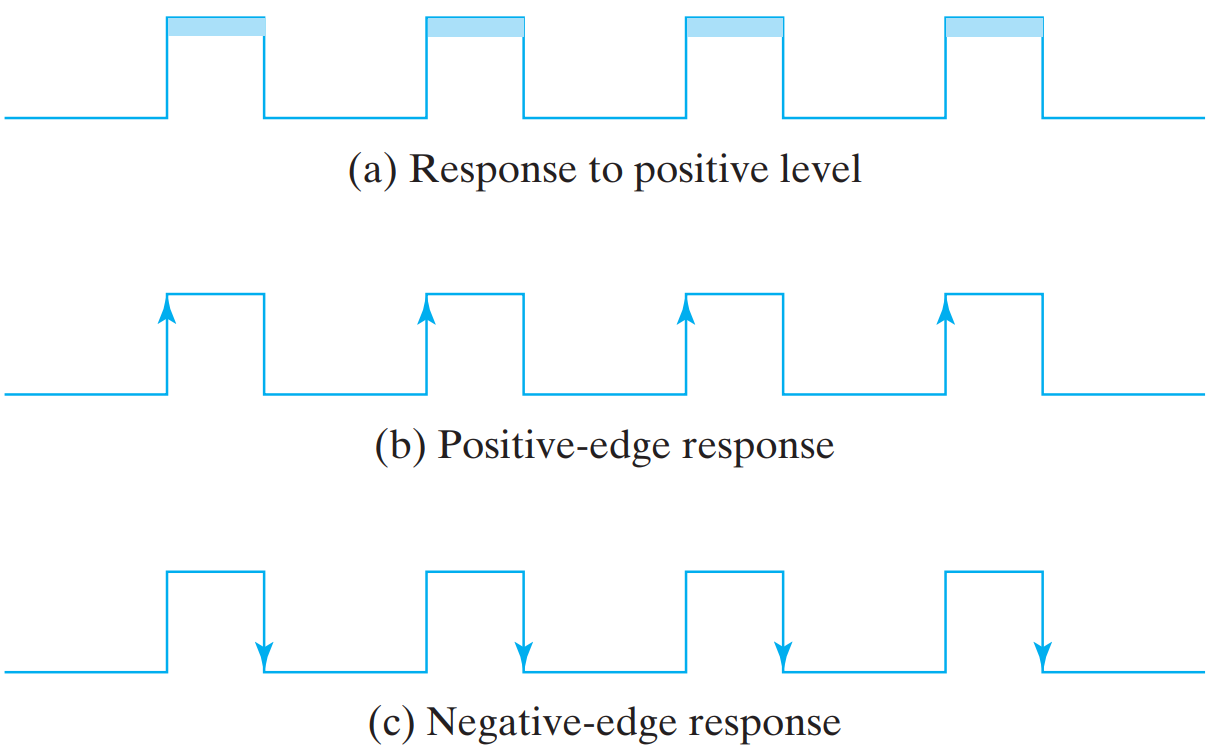
\includegraphics[width=\linewidth]{img/fig-5.8.png}
  \caption{Clock response in latch and flip-flop}
  \label{fig:5.8}
\end{figure}

There are two ways that a latch can be modified to form a flip-flop.
\begin{itemize}
  \item One way is to employ two latches in a special configuration that isolates the output of the flip-flop and prevents it from being affected while the input to the flip-flop is changing.
  \item Another way is to produce a flip-flop that triggers only during a signal transition (from 0 to 1 or from 1 to 0) of the synchronizing signal (clock) and is disabled during the rest of the clock pulse.
\end{itemize}

\subsection{Edge-Triggered D Flip-Flop}
\label{subsec:edge-trig-d-flip-flop}

The construction of a $D$ flip-flop with two $D$ latches and an inverter is shown in Fig. 9. It is often referred to as a master–slave flip-flop. The circuit samples the $D$ input and changes its output $Q$ \textit{only at the negative edge} of the synchronizing or controlling clock.
\begin{figure}[H]
  \centering
  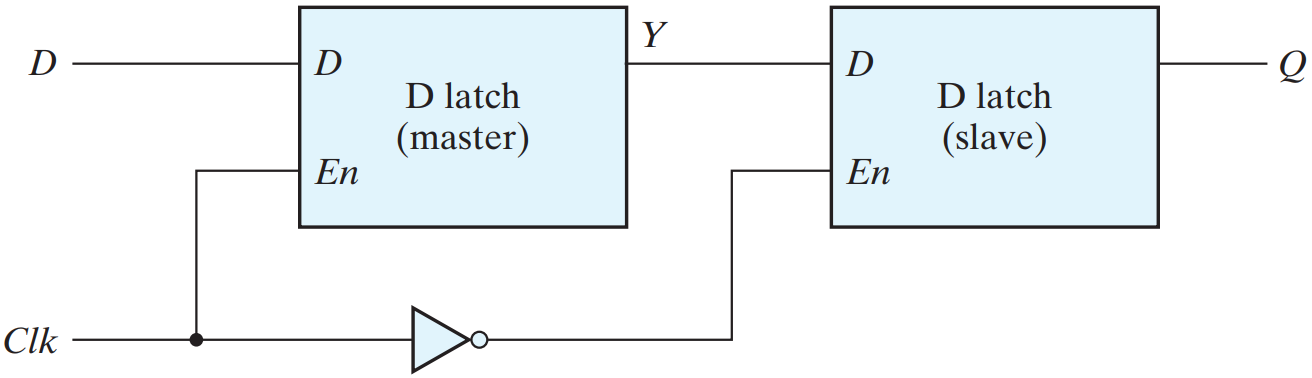
\includegraphics[width=\linewidth]{img/fig-5.9.png}
  \caption{Master–slave $D$ flip-flop}
  \label{fig:5.9}
\end{figure}
\noindent \textit{A change in the output of the flip-flop can be triggered only by and during the transition of the clock from 1 to 0}.

Another construction of an edge-triggered $D$ flip-flop uses three $SR$ latches as shown in Fig. 10.
\begin{figure}[H]
  \centering
  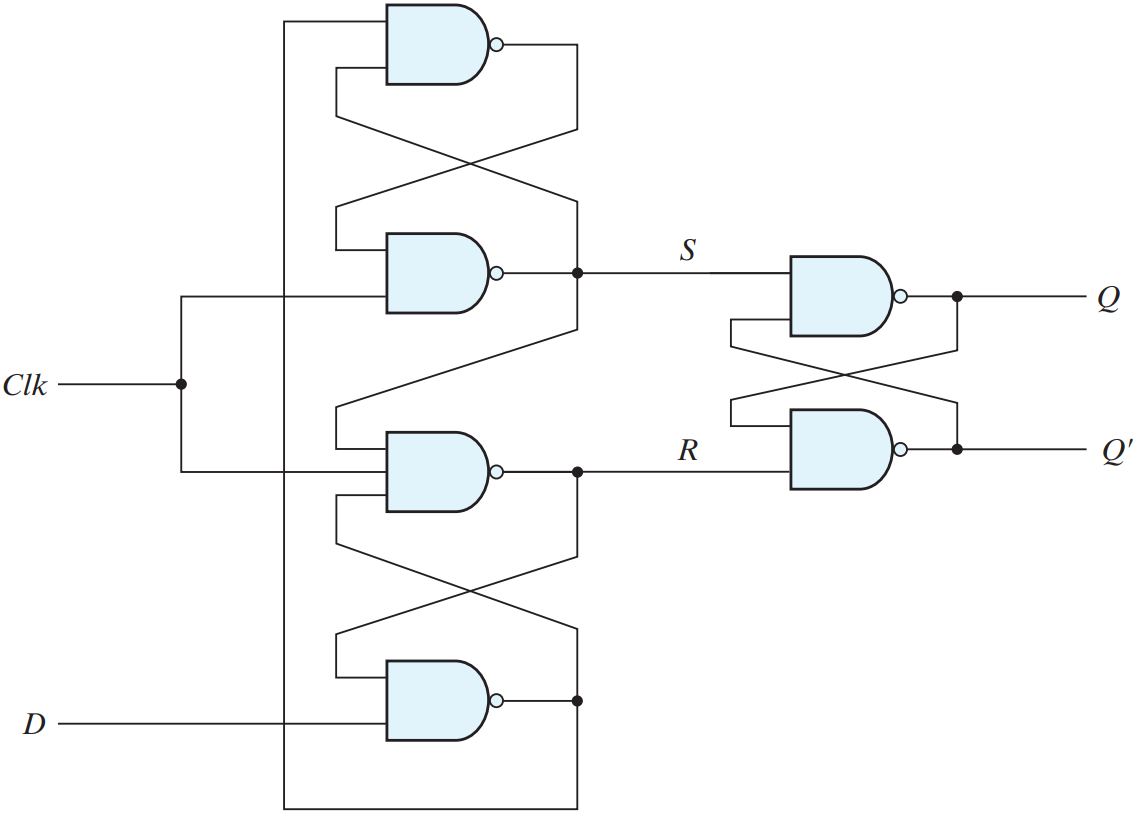
\includegraphics[width=\linewidth]{img/fig-5.10.png}
  \caption{D-type positive-edge-triggered flip-flop}
  \label{fig:5.10}
\end{figure}

The behavior of the master–slave flip-flop just described dictates that
\begin{enumerate}[leftmargin=0.5cm]
  \item The output may change only once,
  \item A change in the output is triggered by the negative edge of the clock,
  \item The change may occur only during the clock's negative level.
\end{enumerate}
\noindent The value that is produced at the output of the flip-flop is the value that was stored in the master stage immediately before the negative edge occurred. It is also possible to design the circuit so that the flip-flop output changes on the positive edge of the clock.

In sum, \textit{when the input clock in the positive-edge-triggered flip-flop makes a positive transition, the value of \textnormal{D} is transferred to \textnormal{Q}}.

The graphic symbol for the edge-triggered $D$ flip-flop is shown in Fig. 11.
\begin{figure}[H]
  \centering
  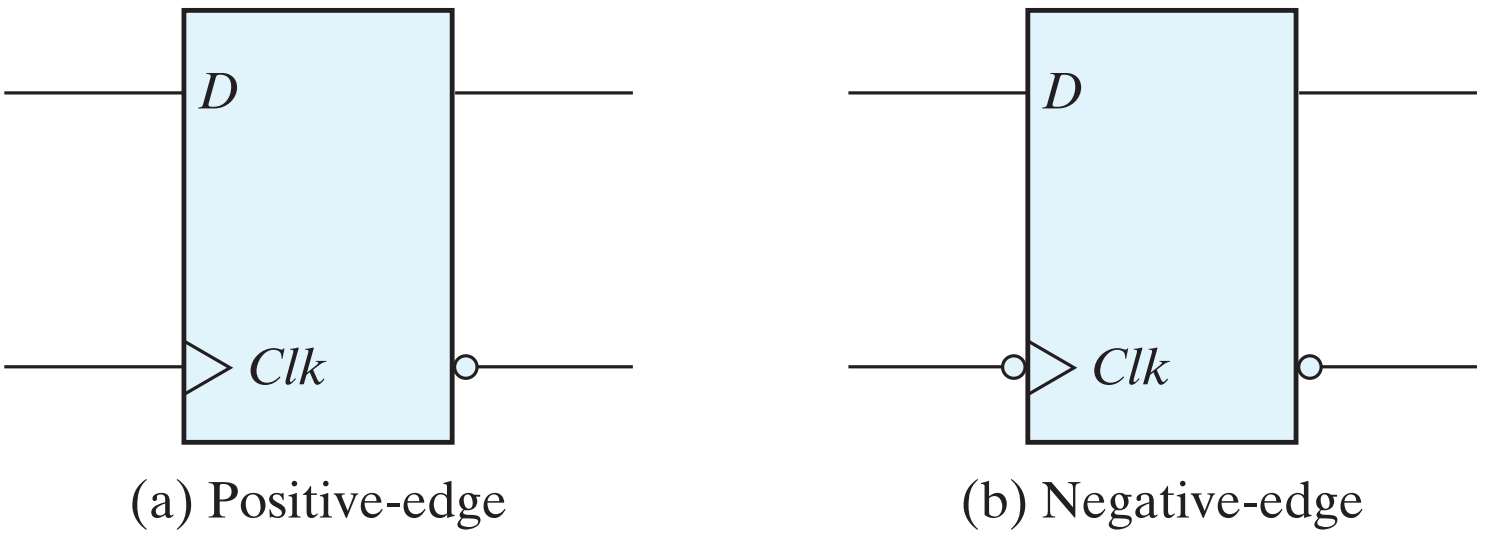
\includegraphics[width=\linewidth]{img/fig-5.11.png}
  \caption{Graphic symbol for edge-triggered D flip-flop}
  \label{fig:5.11}
\end{figure}

\textbf{Note:} A positive-edge flip-flop is one that is activated by the rising (positive) edge of the clock (synchronizing signal).

\subsection{Other Flip-Flops}
\label{subsec:other-flip-flops}

The most economical and efficient flip-flop constructed in this manner is the edge-triggered $D$ flip-flop, because it requires the smallest number of gates. Other types of flip-flops can be constructed by using the $D$ flip-flop and external logic. Two flip-flops less widely used in the design of digital systems are the $JK$ and $T$ flip-flops.

There are three operations that can be performed with a flip-flop:
\begin{enumerate}[]
  \item Set it to 1,
  \item Reset it to 0, or 
  \item Complement its output.
\noindent \end{enumerate}

\subsubsection{JK Flip-Flops}
\label{subsubsec:jk-flip-flops}

With only a single input, the $D$ flip-flop can set or reset the output. The $JK$ flip-flop has two inputs and performs all three operations. The circuit diagram of a $JK$ flip-flop constructed with a $D$ flip-flop 
and gates is shown in Fig. 12(a).
\begin{figure}[H]
  \centering
  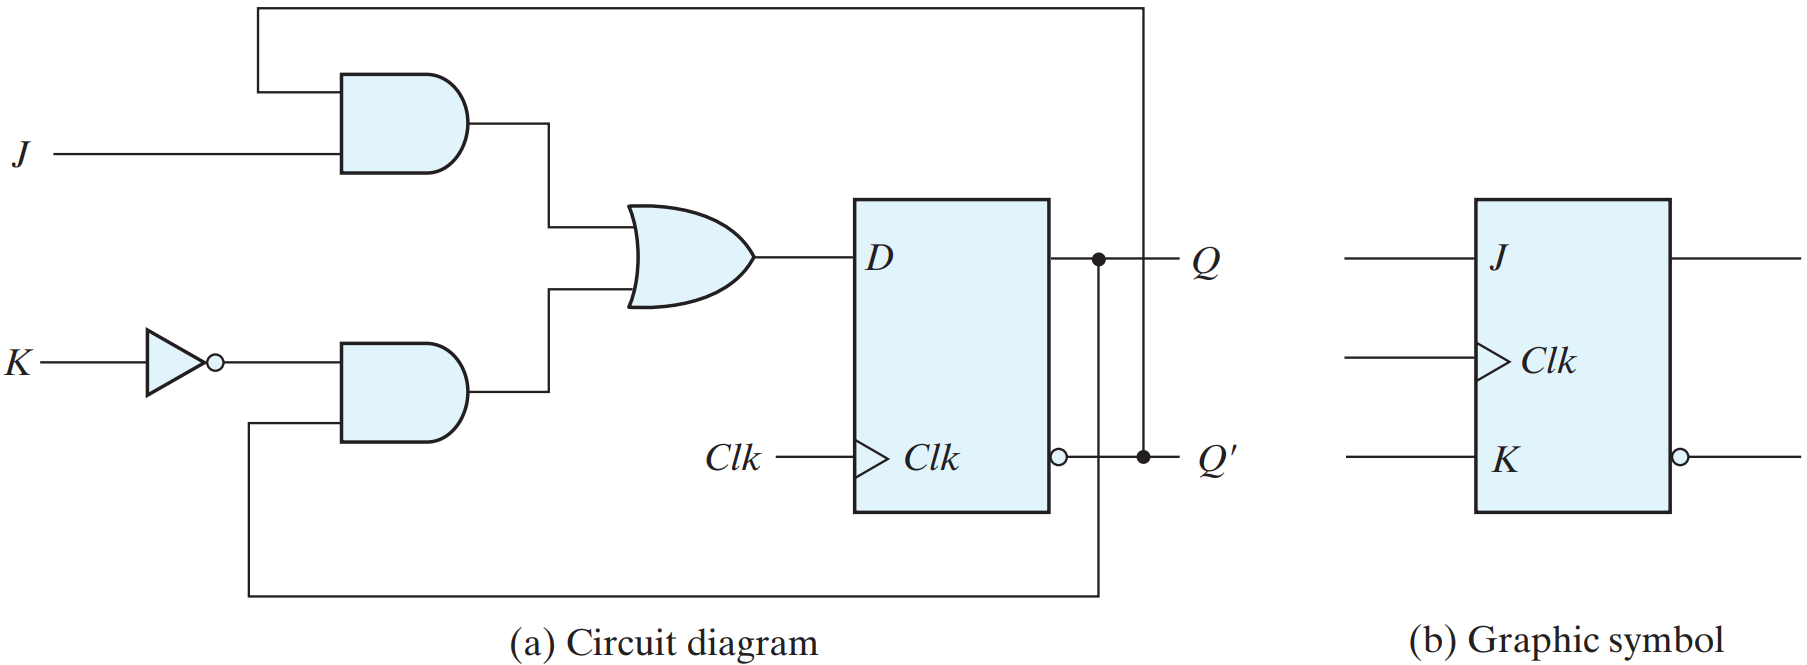
\includegraphics[width=\linewidth]{img/fig-5.12.png}
  \caption{$JK$ flip-flop}
  \label{fig:5.12}
\end{figure}
\noindent The $J$ input sets the flip-flop to 1, the $K$ input resets it 
to 0, and when both inputs are enabled, the output is complemented. This can be verified by investigating the circuit applied to the D input:
\begin{equation*}
  D = JQ' + K'Q
\end{equation*}
The graphic symbol for the $JK$ flip-flop is shown in Fig. 12(b).

\vspace*{\fill}
\columnbreak

\subsubsection{T Flip-Flops}
\label{subsubsec:t-flip-flops}

The $T$ (toggle) flip-flop is a complementing flip-flop and can be obtained from a $JK$ flip-flop when inputs $J$ and $K$ are tied together. This is shown in Fig. 13(a).
\begin{figure}[H]
  \centering
  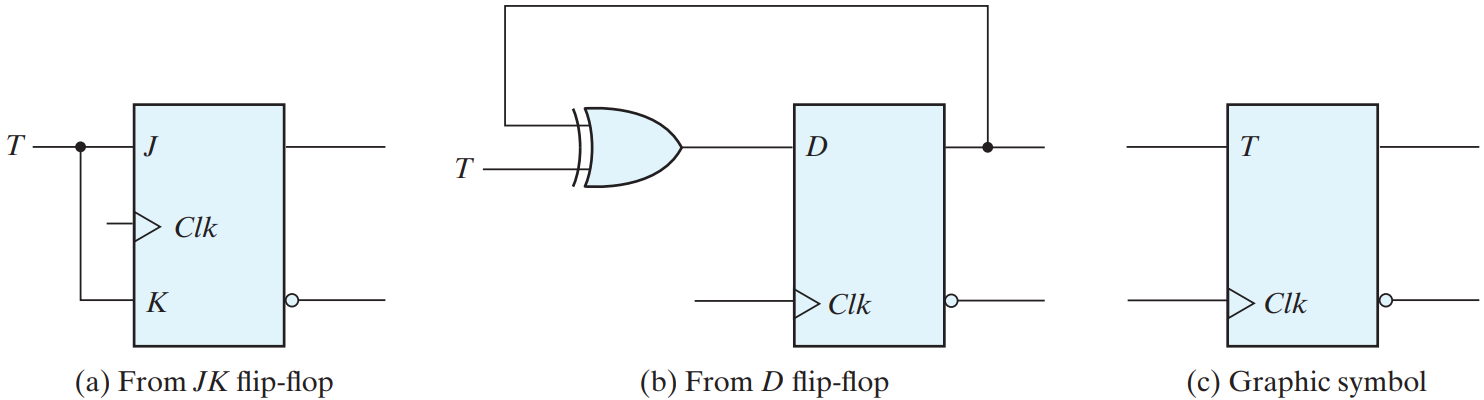
\includegraphics[width=\linewidth]{img/fig-5.13.png}
  \caption{T flip-flop}
  \label{fig:5.13}
\end{figure}
The complementing flip-flop is useful for designing binary counters. The $T$ flip-flop can be constructed with a $D$ flip-flop and an exclusive-OR gate as shown in Fig. 13(b). The expression for the D input is
\begin{equation*}
  D = T \oplus Q = TQ' + T'Q
\end{equation*}
The graphic symbol for this flip-flop has a $T$ symbol in the input.


\subsection{Characteristic Tables}
\label{subsec:char-tables}

The characteristic tables of three types of flip-flops are presented in Table 5.1.
\begin{figure}[H]
  \centering
  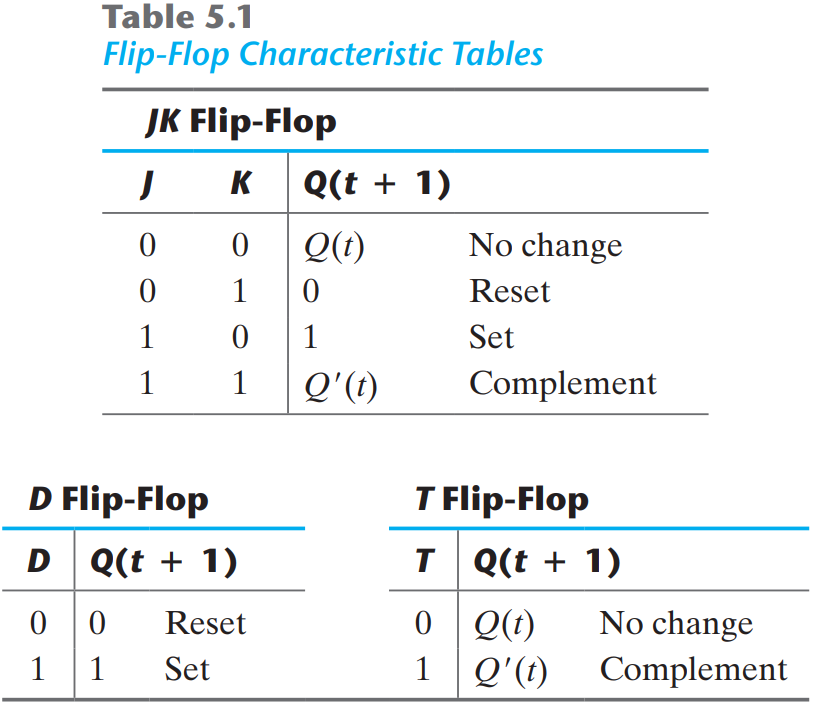
\includegraphics[width=\linewidth]{img/table-5.1.png}
  \label{table:5.1}
\end{figure}


\subsection{Characteristic Equations}
\label{subsec:char-equations}

$D$ flip-flop:
\begin{equation*}
  Q(t + 1) = D
\end{equation*}
$JK$ flip-flop:
\begin{equation*}
  Q(t + 1) = JQ' + K'Q
\end{equation*}
$T$ flip-flop:
\begin{equation*}
  Q(t + 1) = T \oplus Q = TQ' + T'Q
\end{equation*}

\setcounter{figure}{14}
